% Scenario: Ensuring Service Availability During Network Outages
\newcommand{\scenarioOneConcurrency}{
\begin{table}[H]
    \centering
    \begin{tabularx}{\textwidth}{@{} lX @{}}
    \toprule
    \textbf{Aspect} & \textbf{Details} \\
    \midrule
    Source & Network outage impacting the TrIP system's connectivity. \\
    Stimulus & A passenger attempts to validate their ticket at a turnstile during the outage. \\
    Artifact & Hybrid approach of delayed processing and local caching implemented in the TrIP system. \\
    Response & The turnstile, equipped with local caching, validates the passenger's ticket against stored data, allowing entry. Transaction details are queued for delayed processing once network connectivity resumes, ensuring no service disruption. \\
    Measure & Passenger service continuity is maintained with 99.9\% uptime, and ticket validations during outages show no significant delay, ensuring high system availability. \\
    \bottomrule
    \end{tabularx}
    \caption{Scenario for Availability - Network Outage Handling}
    \label{table:availability_network_outage}
\end{table}
}
% Scenario: Maintaining Safety through Authorized Access

\newcommand{\scenarioTwoConcurrency}{
\begin{table}[H]
    \centering
    \begin{tabularx}{\textwidth}{@{} lX @{}}
    \toprule
    \textbf{Aspect} & \textbf{Details} \\
    \midrule
    Source & TrIP system's safety protocols for access control. \\
    Stimulus & An individual attempts to access the transit system without a valid ticket or permission. \\
    Artifact & Turnstile with integrated validation system that checks for valid tickets. \\
    Response & The turnstile denies entry to the individual without a valid ticket, preventing unauthorized access and maintaining the safety and security of the transit environment. \\
    Measure & Zero reported incidents of unauthorized access, ensuring the safety of the transit system and its users. \\
    \bottomrule
    \end{tabularx}
    \caption{Scenario for Safety - Authorized Access Enforcement}
    \label{table:safety_authorized_access}
\end{table}
}

% Scenario: Optimizing Performance with Pre-stored Routes
\newcommand{\scenarioThreeConcurrency}{
\begin{table}[H]
    \centering
    \begin{tabularx}{\textwidth}{@{} lX @{}}
    \toprule
    \textbf{Aspect} & \textbf{Details} \\
    \midrule
    Source & Passenger requests the best route options via the TrIP system during peak hours. \\
    Stimulus & High demand for route information causes potential strain on the system. \\
    Artifact & Optimized Routes Database that stores frequently requested route data. \\
    Response & The TrIP system quickly retrieves optimized route options from the pre-stored data, providing the passenger with fast and efficient service without needing to compute the routes in real-time. \\
    Measure & The response time for route information requests during peak periods remains under 2 seconds, enhancing the overall performance of the system. \\
    \bottomrule
    \end{tabularx}
    \caption{Scenario for Performance - Efficient Route Retrieval}
    \label{table:performance_route_optimization}
\end{table}
}

\section{Concurrency Viewpoint}
We start discussing the information viewpoint by analyzing stakeholder concerns that need to be addressed.
We individuated the following user stories:
\begin{itemize}
    \item User stories TODO
\end{itemize}

As a consequence, we decided to prioritize Quality Attributes for this view as indicated in Table~\ref{tab:concurrency_view}.
\begin{table}[h!]
    \centering
    \resizebox{\textwidth}{!}{%
    \begin{tabular}{|l|c|c|c|c|c|c|c|c|c|}
      \hline
      & Usability & Performance & Security & Modifiability & Cost Efficiency & Availability & Safety & Integrability & Maintainability \\
      \hline
      Concurrency View & 
       & % Usability
      \cellcolor{gray!30}X & % Performance (2nd priority)
       & % Security
       & % Modifiability
       & % Cost Efficiency
      \cellcolor{gray!90}X & % Availability (1st priority)
      \cellcolor{gray!60}X & % Safety
       & % Integrability
       \\ % Maintainability
      \hline
    \end{tabular}
    }
    \caption{Concurrency View Prioritized Quality Attributes}
    \label{tab:concurrency_view}
\end{table}

\subsection{View: Ticket purchase}
\subsubsection{Model}

\begin{figure}[H]
    \centering
    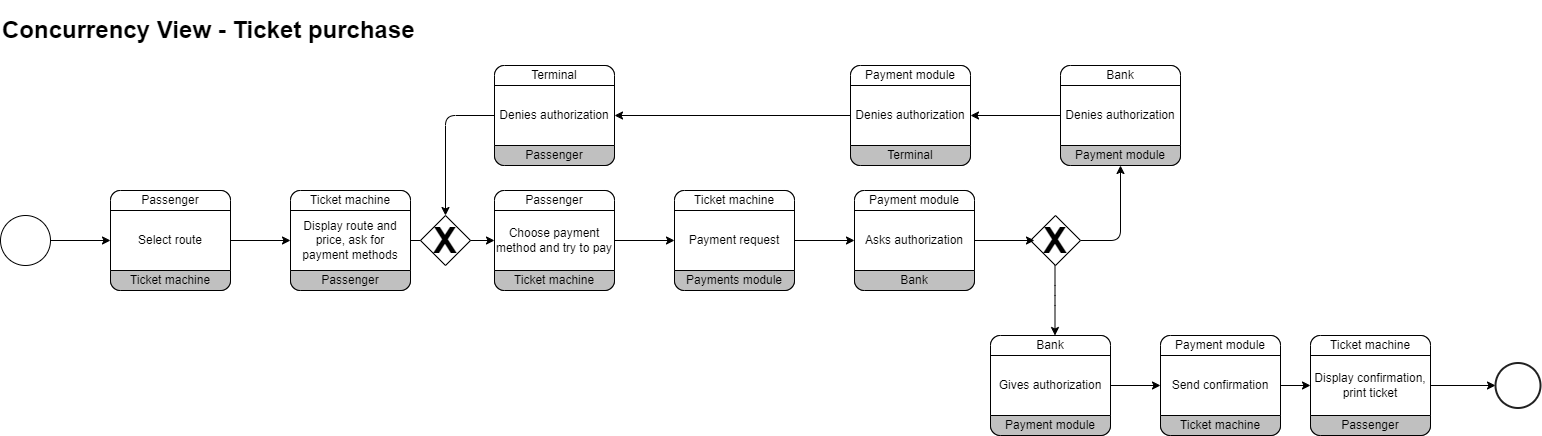
\includegraphics[width=\textwidth]{drawings/views_final_version/concurrency_view_1.png}
    \caption{Concurrency view related to ticket purchase.}
    \label{fig:concurrency_view_1}
\end{figure}

\subsubsection{Description}
In the TRIP SYSTEM, the Passenger starts the process at the Ticket Machine, choosing a route and payment method. The Terminal takes over to process the payment, and the Payment Module communicates with the Bank for payment approval. If the Bank approves, the Payment Module signals the Ticket Machine to confirm the transaction and print the ticket. If the Bank denies the payment, the process is stopped, and the Passenger is notified.

\begin{table}[H]
    \centering
    \caption{Glossary for the Payment and Ticketing Process.}
    \label{tab:payment_ticketing_glossary}
    \begin{tabularx}{\textwidth}{@{}lX@{}} % Use 'X' for auto-adjusting width
    \toprule
    \textbf{Element} & \textbf{Description} \\
    \midrule
    Passenger & The customer who initiates the process by selecting a route and choosing a payment method to pay for a ticket. \\
    Ticket Machine & The interface through which the passenger selects a route, displays the route and price, and chooses a payment method. \\
    Terminal & The point of service where the passenger's payment authorization is processed. \\
    Payment Module & The system component that interacts with the bank to request payment authorization for the transaction. \\
    Bank & The financial institution that either authorizes or denies the payment transaction. \\
    \bottomrule
    \end{tabularx}
\end{table}

\subsubsection{Analysis on Perspectives}
\paragraph{Scenarios}
\scenarioThreeConcurrency

\subsection{View: Scanning procedure}
\subsubsection{Model}
\begin{figure}[H]
    \centering
    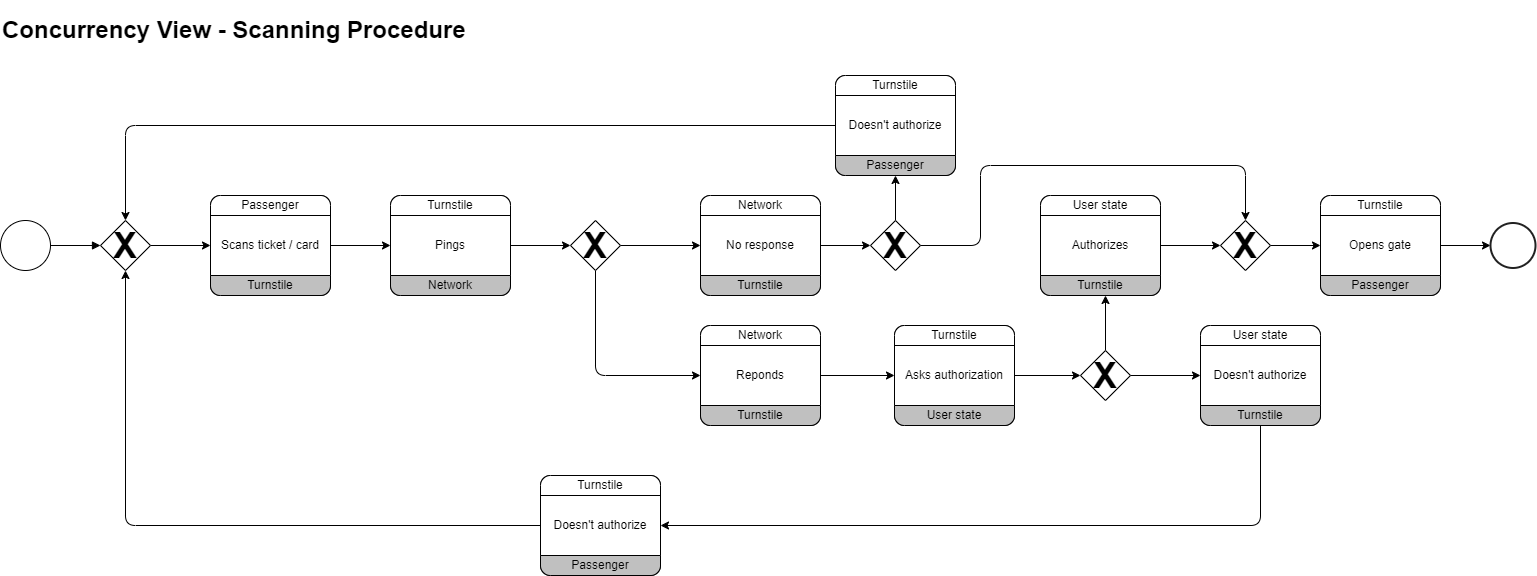
\includegraphics[width=\textwidth]{drawings/views_final_version/concurrency_view_2.png}
    \caption{Concurrency view related to the scanning procedure.}
    \label{fig:concurrency_view_2}
\end{figure}

\subsubsection{Description}
The diagram depicts a turnstile access procedure with conditional paths based on network availability and user authorization. When a Passenger scans their ticket or card at the Turnstile, two scenarios can unfold:

\begin{enumerate}
    \item If the Turnstile is unable to connect to the Network (no response), it defaults to a local decision. In this case, the turnstile can still potentially authorize the passenger to proceed based on offline data or preconfigured rules.
    \item If the Turnstile connects to the Network (network responds), it then requests authorization from the User State. The User State, after evaluating the request, either grants or denies authorization:
    \begin{itemize}
        \item If the User State authorizes the request, the Turnstile receives a signal to open the gate, allowing the Passenger to pass.
        \item If the User State denies the request, the Turnstile will not open, and the Passenger is not allowed to proceed.
    \end{itemize}
\end{enumerate}

This process ensures that the system can function and provide decisions autonomously, even in the absence of network connectivity, enhancing reliability and user experience.

\subsubsection{Glossary of Elements}

\begin{table}[H]
    \centering
    \caption{Glossary for Turnstile Interaction Process.}
    \label{tab:turnstile_interaction_glossary}
    \begin{tabularx}{\textwidth}{@{}lX@{}} % Use 'X' for auto-adjusting width
    \toprule
    \textbf{Component} & \textbf{Description} \\
    \midrule
    Passenger & An individual who is attempting to gain entry through the turnstile by scanning a ticket or card. \\
    Turnstile & A physical barrier at an entry point that controls access, typically based on ticket or card validation. \\
    Network & The communication system that the turnstile interfaces with to verify access rights. \\
    User State & A system component that maintains the current state of a user's access rights, determining whether entry is authorized. \\
    \bottomrule
    \end{tabularx}
\end{table}
\subsubsection{Analysis on Perspectives}
\paragraph{Scenarios}
\scenarioOneConcurrency
\scenarioTwoConcurrency

\subsection{View: Tycoon data updates}
\subsubsection{Model}

\begin{figure}[H]
    \centering
    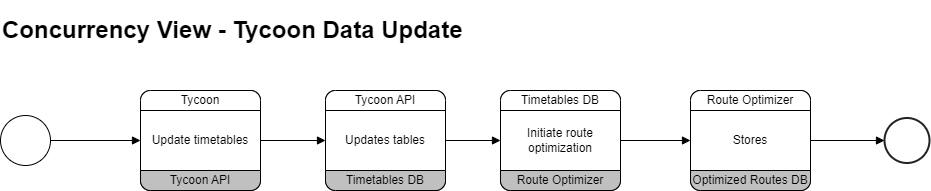
\includegraphics[width=\textwidth]{drawings/views_final_version/concurrency_view_3.png}
    \caption{Concurrency view related to tycoons data updates.}
    \label{fig:concurrency_view_3}
\end{figure}

\subsubsection{Description}
This process outlines how timetable updates and route optimization are handled in the system. It begins with the Tycoon, an administrative role, who updates timetables through the Tycoon API. These updates are then applied to the Timetables DB. Following this update, the Route Optimizer initiates the optimization process, which takes the updated timetable data to determine the most efficient routes. These optimized routes are then stored in the Optimized Routes DB, completing the cycle of updating and optimizing the route information available to the system and its users.

\begin{table}[H]
    \centering
    \caption{Glossary for Route Optimization Process.}
    \label{tab:route_optimization_glossary}
    \begin{tabularx}{\textwidth}{@{}lX@{}} % Use 'X' for auto-adjusting width
    \toprule
    \textbf{Component} & \textbf{Description} \\
    \midrule
    Tycoon & Represents the train companies or transport entities responsible for managing train schedules and routes. \\
    Tycoon API & The application programming interface that allows the tycoons to update and access timetable information. \\
    Timetables DB & The database where train schedules, routes, and associated data are stored and updated. \\
    Route Optimizer & The system component that calculates the most efficient routes, likely using algorithms to process timetable data. \\
    Optimized Routes DB & A specialized database that stores the results of the route optimization process. \\
    \bottomrule
    \end{tabularx}
\end{table}
\subsubsection{Glossary of Elements}

\subsubsection{Analysis on Perspectives}

\paragraph{Scenarios}

The Concurrency Viewpoint is central to the TRiP system's architecture, focusing on ensuring that user interactions with the system occur smoothly and without delay, even when multiple operations are executed simultaneously. This viewpoint addresses the system's capacity to manage concurrent actions effectively, with a particular emphasis on maintaining performance, safety, and availability. \\

\noindent\textbf{Ticket Purchasing Process:} \\
The sequence begins with the passenger selecting a route and payment method via the Ticket Machine. This process is crucial for performance, as it demands a fast and seamless operation to prevent queues and delays. Once the payment method is chosen, the Terminal communicates with the Payment Module to process the transaction. The Payment Module's role here is two-fold: to ensure the safety of the transaction by validating payment with the bank and to maintain the system's performance by providing quick feedback to the Terminal. If the bank authorizes the payment, the Payment Module prompts the Ticket Machine to dispense a ticket, showcasing the system's availability to complete transactions without delay. In case of a denial, the passenger is promptly informed, allowing them to take alternative actions, which is vital for maintaining system usability and ensuring the passenger's experience remains positive. \\

\noindent \textbf{Turnstile Access Control:} \\
The second aspect of concurrency comes into play at the turnstiles, where passengers scan their tickets or cards to gain access to the transport services. In this operation, the system's availability and safety are the primary concerns. The Turnstile must quickly authorize entry to avoid creating bottlenecks, which it does by pinging the Network to retrieve the User State information. If the Network is unresponsive, the Turnstile uses locally cached data to make an authorization decision, ensuring continuous operation and thus maintaining high availability. When the Network responds, the User State determines access permission. This dual approach ensures that access control is robust against network issues, preserving the integrity of operations and passenger safety by preventing unauthorized access. \\

\noindent \textbf{Route Optimization Updates:} \\
Finally, the system’s capacity to update and optimize routes through the Tycoon API and Route Optimizer reflects its modifiability and performance attributes. Tycoons can update timetables, which are then processed to optimize routes, and these optimizations are stored in the Optimized Routes DB for quick retrieval. This ensures that passengers receive up-to-date and efficient routing information, which is especially important during peak traffic conditions. \\

By detailing these processes, the concurrency viewpoint showcases the TrIP system's capability to maintain a high level of service and security across its operations, aligning with the defined quality attributes of performance, safety, and availability.